% !TEX root = ../../main.tex
\chapter{Solutions to exercises}
\label{ch:appendix:exercise-solutions}

Each problem is repeated before its solution, in the order of the exercises
in the main text. Each exercise number links back to the original exercise; the
margin link beside that exercise returns to its entry here.

\section{Sets and foundations of real analysis}
\label{sec:appendix:foundations-solutions}

\solutionheading{hw01:de-morgan}
\begin{restatedproblem}
  % !TEX root = ../../hw01.tex
% Homework 01, Exercise 1. Shared problem statement.
\begin{exercise}
  \label{ex:hw01:de-morgan}
  \solutionlink{hw01:de-morgan}
  Let $\{A_\gamma \mid \gamma \in \Gamma\}$ be a collection of sets.
  Prove De Morgan's laws
  \[
    \begin{aligned}
      \left(\bigcup_{\gamma\in\Gamma} A_\gamma\right)^c
        &= \bigcap_{\gamma\in\Gamma} A_\gamma^c,\\
      \left(\bigcap_{\gamma\in\Gamma} A_\gamma\right)^c
        &= \bigcup_{\gamma\in\Gamma} A_\gamma^c.
    \end{aligned}
  \]
\end{exercise}

\end{restatedproblem}
% !TEX root = ../../hw01.tex
% Homework 01, Exercise 1. Shared solution.

% Transcribed from IMG_8995 and the left page of IMG_8996.
\begin{proof}[Solution]
Fix a set $S$ such that $A_\gamma\subseteq S$ for every
$\gamma\in\Gamma$. All complements in this proof are taken
relative to $S$, so
\[
  A_\gamma^c=S\setminus A_\gamma.
\]
Suppose first that $\Gamma$ is nonempty. We prove each identity
by showing both inclusions.

\begin{marginfigure}
  \centering
  % !TEX root = ../../problems/hw01.tex
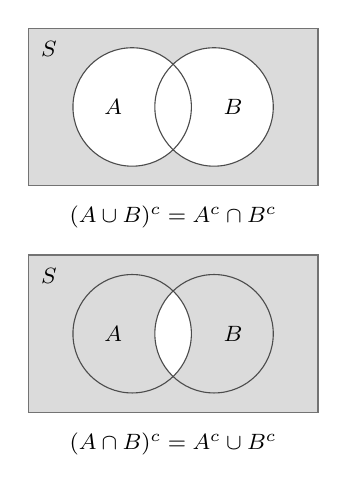
\begin{tikzpicture}[x=0.8cm,y=0.8cm,font=\footnotesize]
  \foreach \offset in {0,-3.6} {
    \begin{scope}[shift={(0,\offset)}]
      \fill[black!14] (0,0) rectangle (4.6,2.5);
    \end{scope}
  }
  % Removing both discs leaves the complement of their union.
  \fill[white] (1.65,1.25) circle[radius=0.94];
  \fill[white] (2.95,1.25) circle[radius=0.94];
  % Removing only the lens leaves the complement of the intersection.
  \begin{scope}[shift={(0,-3.6)}]
    \clip (1.65,1.25) circle[radius=0.94];
    \fill[white] (2.95,1.25) circle[radius=0.94];
  \end{scope}
  \foreach \offset in {0,-3.6} {
    \begin{scope}[shift={(0,\offset)}]
      \draw[black!55] (0,0) rectangle (4.6,2.5);
      \draw[black!70] (1.65,1.25) circle[radius=0.94];
      \draw[black!70] (2.95,1.25) circle[radius=0.94];
      \node at (1.35,1.25) {$A$};
      \node at (3.25,1.25) {$B$};
      \node[anchor=north west] at (0.05,2.45) {$S$};
    \end{scope}
  }
  \node at (2.3,-0.5) {$(A\cup B)^c=A^c\cap B^c$};
  \node at (2.3,-4.1) {$(A\cap B)^c=A^c\cup B^c$};
\end{tikzpicture}

  \caption[De Morgan's laws.]{The upper shaded region lies outside both sets.
    In the lower panel, only the overlap is excluded. All complements
    are taken within the rectangle $S$.}
  \label{fig:hw01:de-morgan}
\end{marginfigure}

\textit{The complement of the union.}
Suppose that
\[
  x\in\left(\bigcup_{\gamma\in\Gamma}A_\gamma\right)^c.
\]
Then $x\in S$ and $x$ does not belong to the union.
If $x$ belonged to any $A_\gamma$, it would belong to the union.
Therefore $x\notin A_\gamma$ for every $\gamma\in\Gamma$.
Since $x\in S$, this gives $x\in A_\gamma^c$ for every $\gamma$,
and hence
\[
  x\in\bigcap_{\gamma\in\Gamma}A_\gamma^c.
\]

Conversely, suppose that
\[
  x\in\bigcap_{\gamma\in\Gamma}A_\gamma^c.
\]
Then $x\in S$ and $x\notin A_\gamma$ for every $\gamma\in\Gamma$.
Thus no member of the family contains $x$, so $x$ does not belong
to their union. Consequently,
\[
  x\in\left(\bigcup_{\gamma\in\Gamma}A_\gamma\right)^c.
\]
Both inclusions hold, proving the first equality.

\handoutonly{\clearpage}

\textit{The complement of the intersection.}
Suppose that
\[
  x\in\left(\bigcap_{\gamma\in\Gamma}A_\gamma\right)^c.
\]
Then $x\in S$ and $x$ does not belong to the intersection.
There must be an index $\gamma_0\in\Gamma$ for which
$x\notin A_{\gamma_0}$. Otherwise, $x$ would belong to every
$A_\gamma$ and therefore to their intersection.
Thus $x\in A_{\gamma_0}^c$, which gives
\[
  x\in\bigcup_{\gamma\in\Gamma}A_\gamma^c.
\]

Conversely, suppose that
\[
  x\in\bigcup_{\gamma\in\Gamma}A_\gamma^c.
\]
Then $x\in A_{\gamma_0}^c$ for at least one index $\gamma_0$.
Hence $x\in S$ and $x\notin A_{\gamma_0}$.
Since $x$ fails to belong to this member of the family, it cannot
belong to the intersection. Thus
\[
  x\in\left(\bigcap_{\gamma\in\Gamma}A_\gamma\right)^c.
\]
Both inclusions hold, proving the second equality.

If $\Gamma$ is empty, we use the relative conventions
\[
  \begin{aligned}
    \bigcup_{\gamma\in\varnothing}A_\gamma&=\varnothing,\\
    \bigcap_{\gamma\in\varnothing}A_\gamma&=S.
  \end{aligned}
\]
Both identities then follow from $\varnothing^c=S$ and $S^c=\varnothing$.

\autoref{fig:hw01:de-morgan} illustrates the difference for two sets.
An element outside their intersection may still belong to one
of the sets. It simply cannot belong to both.
\end{proof}


\solutionheading{hw01:countable-union}
\begin{restatedproblem}
  % !TEX root = ../../hw01.tex
% Homework 01, Exercise 10. Shared problem statement.
\begin{exercise}
  \label{ex:hw01:countable-union}
  \solutionlink{hw01:countable-union}
  Let $A_n$ be a set such that $|A_n|=\aleph_0$ for $n=1,2,\ldots$.
  Prove $|A|=\aleph_0$ where
  \[
    A=\bigcup_{n=1}^{\infty} A_n.
  \]
\end{exercise}

\end{restatedproblem}
% !TEX root = ../../hw01.tex
% Homework 01, Exercise 10. Shared solution.

\begin{proof}[Solution]
Since each $A_n$ is countably infinite, there exists a bijection
from $\N$ to $A_n$. Using the axiom of countable choice, select
one such bijection for each $n$. This gives a list without
repetition within each row, which we write as
\[
  A_n=\{a_{n,1},a_{n,2},a_{n,3},\ldots\}.
\]
Put these lists into rows. Reading one whole row first would
never reach the next row. Instead, follow successive diagonals
$n+m=2,3,\ldots$, alternating direction as in
Figure~\ref{fig:hw01:diagonal-enumeration}. This gives
\[
  a_{1,1},\ a_{1,2},\ a_{2,1},\ a_{3,1},
  \ a_{2,2},\ a_{1,3},\ a_{1,4},\ldots.
\]

\begin{figure}[h]
  \centering
  % !TEX root = ../../problems/hw01.tex
\begin{tikzpicture}[x=1.85cm,y=0.72cm,>=Stealth,font=\small]
  \foreach \col in {1,2,3,4} {
    \node[font=\footnotesize] at (\col,0.75) {$m=\col$};
    \node at (\col,-4) {$\vdots$};
  }
  \foreach \row in {1,2,3,4} {
    \node[anchor=east] at (0.4,{1-\row}) {$A_{\row}$};
    \node at (4.75,{1-\row}) {$\cdots$};
    \foreach \col in {1,2,3,4}
      \node (a\row\col) at (\col,{1-\row}) {$a_{\row,\col}$};
  }
  \node at (4.75,-4) {$\ddots$};
  \foreach \from/\to in {11/12,12/21,21/31,31/22,22/13,
    13/14,14/23,23/32,32/41} {
    \draw[->,black!60,line width=0.85pt,shorten <=2pt,shorten >=2pt]
      (a\from) -- (a\to);
  }
  \draw[->,black!60,line width=0.85pt]
    (a41.south) -- (1,-3.7);
\end{tikzpicture}

  \caption[Enumerating a countable union.]{Follow the arrows along diagonals of constant $n+m$.
    Every entry is reached after finitely many steps.}
  \label{fig:hw01:diagonal-enumeration}
\end{figure}

Each diagonal is finite, and each $a_{n,m}$ has only finitely
many diagonals before its own. Hence every entry is eventually
reached. Every element of $A$ occurs in some row, so this sequence
contains all of $A$.

The sets may overlap. Skip any value already listed, keeping only
its first occurrence. Every element has a first occurrence at
a finite position, so none is lost by this procedure. The
retained list contains each element of $A$ exactly once.
Since $A_1\subseteq A$ is infinite, the retained list is also
infinite. Numbering its entries in order gives a bijection
from $\N$ to $A$. Therefore
\[
  |A|=\aleph_0.\qedhere
\]
\end{proof}


\solutionheading{hw01:prime-roots}
\begin{restatedproblem}
  % !TEX root = ../../hw01.tex
% Homework 01, Exercise 3. Shared problem statement.
\begin{exercise}
  \label{ex:hw01:prime-roots}
  \solutionlink{hw01:prime-roots}
  Let $p=2,3,5,\ldots$ be a prime. Prove that $\sqrt{p}$ is irrational.
  Can this result be extended to $p^{\frac{1}{k}}$ for any integer $k\geq 2$?
\end{exercise}

\end{restatedproblem}
% !TEX root = ../../hw01.tex
% Homework 01, Exercise 3. Shared solution.

% Transcribed from IMG_8997 and the upper left page of IMG_8998.
\begin{proof}[Solution]
We use Euclid's lemma, which states that if a prime divides a
product of integers, it divides at least one factor. Applying this
repeatedly shows that $p\mid a^k$ implies $p\mid a$ for every
positive integer $k$.

\textit{The square root.}
Suppose, for a contradiction, that $\sqrt p\in\Q$. Write
\[
  \sqrt p=\frac ab,
  \qquad a,b\in\Z,\quad b>0,\quad\gcd(a,b)=1.
\]
Squaring gives $a^2=pb^2$, so $p\mid a^2$.
Euclid's lemma gives $p\mid a$, and we can write $a=pm$
for some $m\in\Z$. Substituting and cancelling one factor of $p$ gives
\[
  p^2m^2=pb^2
  \quad\Longrightarrow\quad
  pm^2=b^2.
\]
Hence $p\mid b^2$, so Euclid's lemma also gives $p\mid b$.
The prime $p>1$ therefore divides both $a$ and $b$,
contradicting $\gcd(a,b)=1$. Thus $\sqrt p$ is irrational.

\textit{The general $k$th root.}
Let $k\ge2$ and suppose that $p^{1/k}=a/b$ in lowest terms,
with $a,b\in\Z$ and $b>0$. Raising both sides to the $k$th
power gives $a^k=pb^k$. Thus $p\mid a^k$, and Euclid's lemma
gives $p\mid a$. Writing $a=pm$, we obtain
\[
  p^km^k=pb^k
  \quad\Longrightarrow\quad
  p^{k-1}m^k=b^k.
\]
Since $k-1\ge1$, this shows that $p\mid b^k$, so $p\mid b$.
Again, $p$ divides both $a$ and $b$, contradicting that the
fraction is in lowest terms. Therefore $p^{1/k}$ is irrational
for every integer $k\ge2$.
\end{proof}


\solutionheading{hw01:power-set}
\begin{restatedproblem}
  % !TEX root = ../../hw01.tex
% Homework 01, Exercise 2. Shared problem statement.
\begin{exercise}
  \label{ex:hw01:power-set}
  \solutionlink{hw01:power-set}
  List all the elements in the set $\mathcal{P}(\mathcal{P}(\varnothing))$
  and verify the cardinality formula.
\end{exercise}

\end{restatedproblem}
% !TEX root = ../../hw01.tex
% Homework 01, Exercise 2. Shared solution.

% Transcribed from the right page of IMG_8996.
\begin{proof}[Solution]
The power set is the set of all subsets. The empty set has exactly
one subset, itself, so
\[
  \mathcal{P}(\varnothing)=\{\varnothing\}.
\]
Taking the power set once more gives
\[
  \mathcal{P}(\mathcal{P}(\varnothing))
    =\{\varnothing,\{\varnothing\}\}.
\]
Its elements are the empty set and the singleton containing the empty
set. These are distinct. Since $|\mathcal{P}(\varnothing)|=1$, the
cardinality formula gives
\[
  |\mathcal{P}(\mathcal{P}(\varnothing))|
    =2^{|\mathcal{P}(\varnothing)|}=2^1=2.\qedhere
\]
\end{proof}


\solutionheading{hw01:interval-to-reals}
\begin{restatedproblem}
  % !TEX root = ../../hw01.tex
% Homework 01, Exercise 4. Shared problem statement.
\begin{exercise}
  \label{ex:hw01:interval-to-reals}
  \solutionlink{hw01:interval-to-reals}
  Obtain a bijective map from $(0,1)$ to $\mathbb{R}$.
\end{exercise}

\end{restatedproblem}
% !TEX root = ../../hw01.tex
% Homework 01, Exercise 4. Shared solution.

% Transcribed from the lower left and upper right pages of IMG_8998.
\begin{proof}[Solution]
A map from $A$ to $B$ is a bijection if it is both one-to-one
and onto. This means that every element of $B$ is the image of
exactly one element of $A$.
\autoref{fig:hw01:bijections} contrasts bijections with a map
that fails both conditions.

\begin{figure}[h]
  \centering
  % !TEX root = ../../problems/hw01.tex
% Editable reconstruction of the finite-set mapping sketches in IMG_8998.
\begin{tikzpicture}[x=0.9cm,y=0.9cm,>=Stealth,font=\small]
  \foreach \panel/\captiontext in {0/{Bijection},3.8/{Bijection},7.6/{Not a bijection}} {
    \begin{scope}[shift={(\panel,0)}]
      \draw[black!55] (0,0) ellipse[x radius=0.4,y radius=1.05];
      \draw[black!55] (2.1,0) ellipse[x radius=0.4,y radius=1.05];
      \node at (0,1.35) {$A$};
      \node at (2.1,1.35) {$B$};
      \foreach \y in {-0.65,0,0.65} {
        \fill (0,\y) circle[radius=1.5pt];
        \fill (2.1,\y) circle[radius=1.5pt];
      }
      \node[font=\footnotesize] at (1.05,-1.4) {\captiontext};
    \end{scope}
  }
  \foreach \y in {-0.65,0,0.65}
    \draw[->,shorten <=3pt,shorten >=3pt] (0,\y) -- (2.1,\y);
  \draw[->,shorten <=3pt,shorten >=3pt] (3.8,0.65) -- (5.9,-0.65);
  \draw[->,shorten <=3pt,shorten >=3pt] (3.8,0) -- (5.9,0.65);
  \draw[->,shorten <=3pt,shorten >=3pt] (3.8,-0.65) -- (5.9,0);
  \draw[->,shorten <=3pt,shorten >=3pt] (7.6,0.65) -- (9.7,0.65);
  \draw[->,shorten <=3pt,shorten >=3pt] (7.6,0) -- (9.7,0.65);
  \draw[->,shorten <=3pt,shorten >=3pt] (7.6,-0.65) -- (9.7,-0.65);
\end{tikzpicture}

  \caption[Examples of bijections.]{The first two maps are bijections. The third map is neither
    one-to-one nor onto. Crossing arrows do not prevent a map from
    being bijective.}
  \label{fig:hw01:bijections}
\end{figure}

The tangent function is a bijection from
$(-\pi/2,\pi/2)$ onto $\R$. To use it on $(0,1)$, we first
multiply the input by $\pi$ and then subtract $\pi/2$.
These steps give the composition
\[
  (0,1)\xrightarrow{\,\times\pi\,}(0,\pi)
    \xrightarrow{\,-\pi/2\,}
    \left(-\frac\pi2,\frac\pi2\right)
    \xrightarrow{\,\tan\,}\R.
\]
We can therefore define
\[
  f(x)=\tan\left(\pi x-\frac\pi2\right),
    \qquad 0<x<1.
\]
For $0<x<1$, the angle $\pi x-\pi/2$ lies strictly between
$-\pi/2$ and $\pi/2$, so $f(x)$ is defined and real.
We verify bijectivity by giving its inverse. For $y\in\R$, put
\[
  g(y)=\frac12+\frac{\arctan y}{\pi}.
\]
Here $\arctan y$ is the unique angle in $(-\pi/2,\pi/2)$
whose tangent is $y$. Thus $0<g(y)<1$, and
\[
  f(g(y))=\tan(\arctan y)=y.
\]
This proves that $f$ is onto. Conversely, for $x\in(0,1)$,
the angle lies in the principal interval, so
\[
  g(f(x))=\frac12+
    \frac{\arctan(\tan(\pi x-\pi/2))}{\pi}=x.
\]
If $f(x_1)=f(x_2)$, applying $g$ gives $x_1=x_2$.
Therefore $f$ is also one-to-one and hence is a bijection.
\handoutonly{\clearpage}

\autoref{fig:hw01:tangent-overview} shows the central branch of
$y=\tan t$ in blue and the transformed graph alongside it.
The horizontal change $x=t/\pi+1/2$ compresses that branch by a
factor of $1/\pi$ and shifts it to the right by $1/2$.
Its domain becomes $(0,1)$, while its range remains all of $\R$.

\begin{figure*}[h]
  \centering
  % !TEX root = ../../problems/hw01.tex
% The tangent overview and its transformed central branch share one figure.
\begin{tikzpicture}[>=Stealth,font=\footnotesize]
  \definecolor{tangentblue}{HTML}{69B4E4}
  \definecolor{tangentwash}{HTML}{EAF6FD}

  \begin{scope}[x=0.62cm,y=0.42cm]
    \fill[tangentwash] (-1.5708,-4.6) rectangle (1.5708,4.6);
    \foreach \boundary in {-2.5,-1.5,1.5,2.5} {
      \draw[dashed,black!30] ({\boundary*pi},-4.6)
        -- ({\boundary*pi},4.6);
    }
    \foreach \boundary in {-0.5,0.5} {
      \draw[dashed,tangentblue] ({\boundary*pi},-4.6)
        -- ({\boundary*pi},4.6);
    }
    \draw[->,black!65] (-8.15,0) -- (8.3,0) node[right] {$t$};
    \draw[->,black!65] (0,-4.85) -- (0,5.05) node[above] {$y$};

    % Sample each branch separately, away from the vertical asymptotes.
    \foreach \period in {-2,-1,1,2} {
      \draw[thick,black!65,<->,domain=-1.347:1.347,samples=121,smooth]
        plot ({\x+\period*pi},{tan(deg(\x))});
    }
    \draw[line width=1.3pt,tangentblue,<->,
      domain=-1.347:1.347,samples=121,smooth]
      plot (\x,{tan(deg(\x))});

    \foreach \period/\ticktext in {-2/{-2\pi},-1/{-\pi},1/{\pi},2/{2\pi}} {
      \draw[black!65] ({\period*pi},0.12) -- ({\period*pi},-0.12);
      \node[below,fill=white,inner sep=2pt]
        at ({\period*pi},-0.14) {$\ticktext$};
    }
    \node[below right,inner sep=2pt] at (0,0) {$0$};
    \foreach \level in {-4,-2,2,4} {
      \draw[black!65] (-0.09,\level) -- (0.09,\level);
      \node[left,inner sep=2pt] at (-0.09,\level) {$\level$};
    }
    \foreach \boundary/\ticktext in {
      -2.5/{-5\pi/2},-1.5/{-3\pi/2},-0.5/{-\pi/2},
      0.5/{\pi/2},1.5/{3\pi/2},2.5/{5\pi/2}} {
      \node[below] at ({\boundary*pi},-4.85) {$\ticktext$};
    }
    \node at (0,-6.4) {$y=\tan t$};
  \end{scope}

  \begin{scope}[shift={(7.05cm,0)},x=2.75cm,y=0.42cm]
    \draw[dashed,black!45] (1,-4.6) -- (1,4.6);
    \draw[->,black!65] (-0.12,0) -- (1.18,0) node[right] {$x$};
    \draw[->,black!65] (0,-4.85) -- (0,5.05) node[above] {$y$};
    % The same parameter t places the selected branch at x=t/pi+1/2.
    \draw[thick,<->,domain=-1.347:1.347,samples=121,smooth]
      plot ({\x/pi+0.5},{tan(deg(\x))});
    \node[below left,fill=white,inner sep=1pt] at (0,0) {$0$};
    \node[below,fill=white,inner sep=2pt] at (1,0) {$1$};
    \node[below right,fill=white,inner sep=2pt] at (0.5,0) {$\tfrac12$};
    \node at (0.5,-6.4) {$y=\tan(\pi x-\pi/2)$};
  \end{scope}
\end{tikzpicture}

  \caption[Mapping an interval onto the real line.]{The left panel highlights the central tangent branch on
    $(-\pi/2,\pi/2)$. The right panel shows this branch after the
    change of input. The vertical asymptotes now occur at $x=0$
    and $x=1$. The horizontal axes use different scales.}
  \label{fig:hw01:tangent-overview}
\end{figure*}
\end{proof}

% Flush the wide tangent figure before the next margin diagram.
\clearpage

\solutionheading{hw01:open-to-closed-interval}
\begin{restatedproblem}
  % !TEX root = ../../hw01.tex
% Homework 01, Exercise 5. Shared problem statement.
\begin{exercise}
  \label{ex:hw01:open-to-closed-interval}
  \solutionlink{hw01:open-to-closed-interval}
  Obtain a bijective map from $(0,1)$ to $[0,1]$.
\end{exercise}

\end{restatedproblem}
% !TEX root = ../../hw01.tex
% Homework 01, Exercise 5. Shared solution.

% Transcribed from the lower right page of IMG_8998 and left page of IMG_8999.
\begin{proof}[Solution]
The identity $f(x)=x$ maps $(0,1)$ to itself, but it misses the
endpoints of $[0,1]$, as shown in \autoref{fig:hw01:identity-map}.
We can make room for them by moving a countable sequence of points.

First assign
\[
  f\left(\frac12\right)=0,
  \qquad f\left(\frac13\right)=1.
\]
\begin{marginfigure}[12pt]
  \centering
  % !TEX root = ../../problems/hw01.tex
\begin{tikzpicture}[x=2.9cm,y=2.9cm,>=Stealth,font=\footnotesize]
  \draw[->] (-0.12,0) -- (1.14,0) node[right] {$x$};
  \draw[->] (0,-0.12) -- (0,1.14) node[above] {$y$};
  \draw[thick] (0,0) -- (1,1);
  \draw[densely dotted,black!50] (1,0) -- (1,1) -- (0,1);
  \draw[fill=white] (0,0) circle[radius=1.8pt];
  \draw[fill=white] (1,1) circle[radius=1.8pt];
  \node[below left] at (0,0) {$0$};
  \node[below] at (1,0) {$1$};
  \node[left] at (0,1) {$1$};
  \node[above left] at (0.65,0.65) {$y=x$};
\end{tikzpicture}

  \caption[The identity misses the endpoints.]{The identity on $(0,1)$ misses the target values $0$ and $1$.
    Both endpoints of the graph are excluded.}
  \label{fig:hw01:identity-map}
\end{marginfigure}

The values $1/2$ and $1/3$ must now be supplied by other inputs.
We use $1/4$ and $1/5$ for these values, and then continue shifting
the reciprocals to fill the resulting gaps. This gives
\[
  f\left(\frac14\right)=\frac12,\quad
  f\left(\frac15\right)=\frac13,\quad
  f\left(\frac16\right)=\frac14,\quad\ldots
\]
\autoref{fig:hw01:reciprocal-shift} illustrates this shift.
We leave all other points fixed. Define a map $f$ from $(0,1)$
to $[0,1]$ by
\[
  f(x)=
  \begin{cases}
    0, & x=\frac12,\\[2pt]
    1, & x=\frac13,\\[2pt]
    \dfrac1{n-2}, & x=\frac1n,\quad n\in\N,\ n\ge4,\\[4pt]
    x, & \text{otherwise}.
  \end{cases}
\]

\begin{figure}[h]
  \centering
  % !TEX root = ../../problems/hw01.tex
\begin{tikzpicture}[x=0.92cm,y=1cm,>=Stealth,font=\small]
  \node[anchor=east] at (-0.35,1.2) {$x$};
  \node[anchor=east] at (-0.35,0) {$f(x)$};
  \foreach \pos/\source/\target in {
    0.2/{\frac12}/{0},
    1.55/{\frac13}/{1},
    2.9/{\frac14}/{\frac12},
    4.25/{\frac15}/{\frac13},
    5.6/{\frac16}/{\frac14},
    8.4/{\frac1n}/{\frac1{n-2}}} {
    \node at (\pos,1.2) {$\source$};
    \node at (\pos,0) {$\target$};
    \draw[->] (\pos,0.86) -- (\pos,0.35);
  }
  \node at (7,1.2) {$\cdots$};
  \node at (7,0) {$\cdots$};
  \node at (9.55,1.2) {$\cdots$};
  \node at (9.55,0) {$\cdots$};
\end{tikzpicture}

  \caption[Shifting a reciprocal sequence.]{The reciprocal sequence is shifted to accommodate both
    endpoints. Every point outside this sequence remains fixed.}
  \label{fig:hw01:reciprocal-shift}
\end{figure}

To check bijectivity, put
\[
  S=\left\{\frac1n\mid n\in\N,\ n\ge2\right\}.
\]
The cases in the definition are disjoint and cover $(0,1)$.
Every output lies in $[0,1]$, so the function is well-defined.

Among the inputs in $S$, only $1/2$ maps to $0$, and only $1/3$
maps to $1$. For each integer $m\ge2$, solving $1/(n-2)=1/m$
gives the unique input $1/(m+2)$. Thus $f$ maps $S$ bijectively
onto $S\cup\{0,1\}$.

On $(0,1)\setminus S$, the map is the identity, with image
$(0,1)\setminus S$. This image is disjoint from $S\cup\{0,1\}$,
so no fixed point can give a second preimage for a value already
supplied by the reciprocal sequence. Together the two images
cover $[0,1]$. Every target value therefore has exactly one
preimage, proving that $f$ is a bijection.
\end{proof}


\solutionheading{hw01:square-cardinality}
\begin{restatedproblem}
  % !TEX root = ../../hw01.tex
% Homework 01, Exercise 8. Shared problem statement.
\begin{exercise}
  \label{ex:hw01:square-cardinality}
  \solutionlink{hw01:square-cardinality}
  Show that
  \[
    |(0,1)\times(0,1)|=|(0,1)|=\aleph.
  \]
  (\textit{Corrected hint.} For each number in $(0,1)$, choose the decimal
  expansion that is not eventually all $9$s. We can then write
  \[
    x\in(0,1),\quad x=0.x_1x_2\cdots,\quad
    x_i\in\{0,\ldots,9\},\quad i=1,2,\ldots.
  \]
  Then define a map from $(0,1)\times(0,1)$ to $(0,1)$ by
  \[
    (x,y)=(0.x_1x_2\cdots,0.y_1y_2\cdots)
    \mapsto (0.x_1y_1x_2y_2\ldots)=z\in(0,1).
  \]
  Show that this map is injective, then use injections in both directions.)
\end{exercise}

\end{restatedproblem}
% !TEX root = ../../hw01.tex
% Homework 01, Exercise 8. Shared solution.

\begin{proof}[Solution]
Put $I=(0,1)$. For each number in $I$, we choose the unique
decimal expansion that is not eventually all $9$s.
For example, we write one half as $0.5000\ldots$ instead of
$0.4999\ldots$. Each digit may be any of $0,1,\ldots,9$.

For $x=0.x_1x_2\ldots$ and $y=0.y_1y_2\ldots$, define
\[
  F(x,y)=0.x_1y_1x_2y_2\ldots.
\]
Figure~\ref{fig:hw01:decimal-interleaving} shows how the odd
positions record $x$ and the even positions record $y$.

\begin{figure*}[h]
  \centering
  % !TEX root = ../../problems/hw01.tex
\begin{tikzpicture}[x=1cm,y=1cm,>=Stealth,font=\small]
  \node[anchor=east] at (-0.75,1.25) {$x=0.$};
  \node[anchor=east] at (-0.75,0) {$F(x,y)=0.$};
  \node[anchor=east] at (-0.75,-1.25) {$y=0.$};
  \foreach \index in {1,2,3,4} {
    \pgfmathsetmacro{\oddpos}{3.0*(\index-1)}
    \pgfmathsetmacro{\evenpos}{\oddpos+1.5}
    \node[text=black] (x\index) at (\oddpos,1.25) {$x_{\index}$};
    \node[text=black] (y\index) at (\evenpos,-1.25) {$y_{\index}$};
    \node[fill=black!6,minimum width=0.65cm,minimum height=0.5cm]
      (odd\index) at (\oddpos,0) {$x_{\index}$};
    \node[fill=black!12,minimum width=0.65cm,minimum height=0.5cm]
      (even\index) at (\evenpos,0) {$y_{\index}$};
    \draw[->,black!65] (x\index.south) -- (odd\index.north);
    \draw[->,black!65] (y\index.north) -- (even\index.south);
  }
  \foreach \height in {-1.25,0,1.25}
    \node at (12.0,\height) {$\cdots$};
\end{tikzpicture}

  \caption[Interleaving decimal digits.]{Interleaving keeps both digit sequences. Read the odd
    positions to recover $x$, and the even positions to recover $y$.}
  \label{fig:hw01:decimal-interleaving}
\end{figure*}

\handoutonly{\clearpage}

We first check that this construction gives a number in $I$.
The output digits cannot be eventually all $9$s. Otherwise,
both input expansions would also be eventually all $9$s,
contradicting our choice of decimal expansions.

Since $x>0$, at least one of its digits is nonzero. This digit
occurs in an odd position of the output, so $F(x,y)>0$.
The output is less than $1$ because its digits are not all $9$s.
Therefore $F(x,y)\in I$, and its displayed decimal expansion
follows our convention.

If $F(x,y)=F(u,v)$, uniqueness of the digits gives $x_j=u_j$
and $y_j=v_j$ for every $j$. Hence $x=u$ and $y=v$, so $F$
is one-to-one.

However, $F$ is not onto, despite the claim in the original hint.
To see this, consider $z=0.101010\ldots\in I$.
If $F(x,y)=z$, the even digits would force $y=0.000\ldots=0$.
This is impossible because $0\notin I$, so $z$ has no preimage.

We therefore use an injection in the reverse direction as well.
Define a map $G$ from $I$ to $I\times I$ by
\[
  G(t)=\left(t,\frac12\right).
\]
Both coordinates lie in $I$, so the map is well-defined.
If $G(t)=G(s)$, equality of the first coordinates gives $t=s$.
Hence $G$ is one-to-one.

The Cantor--Schr\"oder--Bernstein theorem says that injections
in both directions imply the existence of a bijection.
Applying it to $F$ and $G$ gives $|I\times I|=|I|$.
By Exercise~\ref{ex:hw01:interval-to-reals}, $|I|=|\R|=\aleph$.
Therefore
\[
  |(0,1)\times(0,1)|=|(0,1)|=\aleph.\qedhere
\]
\end{proof}


\solutionheading{hw01:transcendental-cardinality}
\begin{restatedproblem}
  % !TEX root = ../../hw01.tex
% Homework 01, Exercise 6. Shared problem statement.
\begin{exercise}
  \label{ex:hw01:transcendental-cardinality}
  \solutionlink{hw01:transcendental-cardinality}
  Let $\aleph_0$ and $\aleph$ denote the cardinalities of $\mathbb{N}$ and
  $\mathbb{R}$ respectively. Recall that the Continuum Hypothesis (CH)
  states that there is no cardinality between $\aleph_0$ and $\aleph$.
  Use CH to prove that the set of transcendental numbers, $\mathbb{T}$,
  has the same cardinality $\aleph$ as that of $\mathbb{R}$.
\end{exercise}

\end{restatedproblem}
% !TEX root = ../../hw01.tex
% Homework 01, Exercise 6. Shared solution.

% Completed from the argument on the right page of IMG_8999.
\begin{proof}[Solution]
Let $\mathbb{A}$ be the set of real algebraic numbers and
$\mathbb{T}$ the set of real transcendental numbers. An algebraic
number is a root of a nonzero polynomial with integer coefficients;
a transcendental number is not such a root. Hence
\[
  \R=\mathbb{A}\cup\mathbb{T},
  \qquad\mathbb{A}\cap\mathbb{T}=\varnothing.
\]
First, we show that $\mathbb{A}$ is countable. For each $n\ge1$,
consider the nonzero polynomials
\[
  P(X)=c_0+c_1X+\cdots+c_nX^n,
  \qquad c_j\in\Z,\quad |c_j|\le n.
\]
Each of the $n+1$ coefficients has $2n+1$ possible values, so
there are at most $(2n+1)^{n+1}$ such polynomials.
A nonzero polynomial of degree at most $n$ has at most $n$
distinct real roots. Thus the set $F_n$ of all their real roots
is finite.

Every algebraic number is a root of a nonzero integer polynomial.
Taking $n$ at least as large as its degree and the absolute values
of all its coefficients places that root in $F_n$.
Conversely, every root in $F_n$ is algebraic. Hence
\[
  \mathbb{A}=\bigcup_{n=1}^{\infty}F_n.
\]
Within each finite set $F_n$, list the roots in increasing order.
Read these finite lists in the order $F_1,F_2,\ldots$, skipping
repeated roots. Each root is reached after finitely many steps.
This proves that $\mathbb{A}$ is countable. Every $n\in\N$
is a root of $X-n$, so $\N\subseteq\mathbb{A}$. Thus
$\mathbb{A}$ is infinite, and $|\mathbb{A}|=\aleph_0$.

\begin{marginfigure}
  \centering
  % !TEX root = ../../problems/hw01.tex
\begin{tikzpicture}[x=1cm,y=1cm,>=Stealth,font=\footnotesize]
  \draw[->,black!55] (0,0) -- (3.8,0);
  \draw[black!65,fill=white] (0.25,0) circle[radius=2.5pt];
  \fill (3.45,0) circle[radius=3pt];
  \node[below=6pt] at (0.25,0) {$\aleph_0$};
  \node[below=6pt] at (3.15,0) {$|\mathbb{T}|=\aleph$};
  \node[above=8pt,align=center] at (1.85,0)
    {No intermediate\\cardinality under CH};
\end{tikzpicture}

  \caption[The continuum hypothesis.]{CH excludes intermediate cardinalities. Since
    $\mathbb{T}$ is uncountable and contained in $\R$, its cardinality
    must equal $\aleph$.}
  \label{fig:hw01:continuum-gap}
\end{marginfigure}

Now suppose that $\mathbb{T}$ were countable. Then
$\R=\mathbb{A}\cup\mathbb{T}$ would be a union of two countable
sets and therefore countable. This contradicts the uncountability
of $\R$. Hence $\mathbb{T}$ is uncountable. Since
$\mathbb{T}\subseteq\R$, we have
\[
  \aleph_0<|\mathbb{T}|\le|\R|=\aleph.
\]
By CH there is no cardinality strictly between $\aleph_0$ and
$\aleph$, as illustrated in Figure~\ref{fig:hw01:continuum-gap}.
The lower endpoint is already excluded, so the only possibility is
\[
  |\mathbb{T}|=\aleph.\qedhere
\]
\end{proof}


\solutionheading{hw01:linear-independence}
\begin{restatedproblem}
  % !TEX root = ../../hw01.tex
% Homework 01, Exercise 7. Shared problem statement.
\begin{exercise}
  \label{ex:hw01:linear-independence}
  \solutionlink{hw01:linear-independence}
  Let $\tau$ be a transcendental number whose existence is proven already.
  Show that for any $n\in\mathbb{N}$, the numbers
  \[
    \tau,\ldots,\tau^n
  \]
  are linearly independent over the field $\mathbb{Q}$.

  That is, if there are $r_1,\ldots,r_n\in\mathbb{Q}$ such that
  \[
    r_1\tau+\cdots+r_n\tau^n=0,
  \]
  then $r_1=\cdots=r_n=0$.

  (In the language of Linear Algebra, this result indicates that the set
  $\mathbb{R}$ viewed as a vector space over $\mathbb{Q}$ is infinitely
  dimensional.)
\end{exercise}

\end{restatedproblem}
% !TEX root = ../../hw01.tex
% Homework 01, Exercise 7. Shared solution.

\begin{proof}[Solution]
Suppose that
\[
  r_1\tau+\cdots+r_n\tau^n=0,
  \qquad r_1,\ldots,r_n\in\Q.
\]
We want to show that every coefficient is zero. Suppose, for a
contradiction, that at least one $r_j\ne0$.

Write $r_j=a_j/b_j$, where $a_j\in\Z$ and $b_j\in\N$.
Put $D=b_1\cdots b_n>0$. We multiply through by $D$ to clear
all the denominators and obtain
\[
  (Dr_1)\tau+\cdots+(Dr_n)\tau^n=0.
\]
Each $Dr_j$ is an integer, and at least one is nonzero since
$D\ne0$. Therefore
\[
  P(X)=(Dr_1)X+\cdots+(Dr_n)X^n
\]
is a nonzero polynomial with integer coefficients satisfying
$P(\tau)=0$. This would make $\tau$ algebraic, contradicting
the assumption that it is transcendental.

Thus $r_1=\cdots=r_n=0$. Since $n$ was arbitrary, the numbers
$\tau,\ldots,\tau^n$ are linearly independent over $\Q$ for every
$n\in\N$.
\marginnote{Including a constant term does not change the argument.
  Thus $1,\tau,\ldots,\tau^n$ are also linearly independent over $\Q$.}
\end{proof}


\solutionheading{hw02:newton-iteration}
\begin{restatedproblem}
  % !TEX root = ../../hw02.tex
% Homework 02, Exercise 6. Shared problem statement.
\begingroup
\renewcommand{\labelenumi}{(\alph{enumi})}
\begin{exercise}
  \label{ex:hw02:newton-iteration}
  \solutionlink{hw02:newton-iteration}
  In class, we discussed the iteration process
  \[
    x_{n+1}=a+\frac{1}{x_n},\quad n=0,1,2,\ldots,
    \quad a\geq 1,\quad x_0>0,
  \]
  whose limit gives us the continuous fraction
  \[
    b=a+\frac{1}{a+\frac{1}{a+\frac{1}{a+\cdots}}}.
  \]
  That is, $b$ is a fixed point of the function
  \[
    f(x)=a+\frac{1}{x},\quad x>0,
  \]
  which is realized as a root of the function $F(x)=x-f(x)$ $(x>0)$.
  \begin{enumerate}
    \item Show that the iterative algorithm
      \[
        x_{n+1}=\frac{ax_n^2+2x_n}{1+x_n^2},
        \quad n=0,1,2,\ldots,\quad x_0>0,
      \]
      arises from Newton's method that may be used to approach $b$ of our problem.
    \item Assume that $\{x_n\}$ in (a) converges.
      Verify that the limit is indeed the continuous fraction $b$ defined above.
    \item Take $a=\frac{3}{2}$. Prove $0<x_n\leq 2$ for $n=1,2,\ldots$.
    \item Prove that $\{x_n\}_{n=1,2,\ldots}$ increases for any $x_0\ne 2$
      and is constant when $x_0=2$.
    \item Show that $\{x_n\}$ converges to $2$ with any initial state $x_0$
      (thereby establishing the ``global convergence'' of the algorithm).
  \end{enumerate}
\end{exercise}
\endgroup

\end{restatedproblem}
% !TEX root = ../../hw02.tex
% Homework 02, Exercise 6. Shared solution.
\begingroup
\renewcommand{\labelenumi}{(\alph{enumi})}
\allowdisplaybreaks[1]

\begin{proof}[Solution]
\leavevmode
\begin{enumerate}
  \item \textit{Newton's method.}
    For $x>0$, let
    \[
      F(x)=x-a-\frac1x,\qquad F'(x)=1+\frac1{x^2}>0.
    \]
    Newton's method for $F(x)=0$ is therefore
    \[
      \begin{aligned}
        x_{n+1}
          &=x_n-\frac{F(x_n)}{F'(x_n)}\\
          &=x_n-\frac{x_n-a-1/x_n}{1+1/x_n^2}\\
          &=\frac{x_n(1+x_n^2)-(x_n^3-ax_n^2-x_n)}{1+x_n^2}\\
          &=\frac{ax_n^2+2x_n}{1+x_n^2},
      \end{aligned}
    \]
    which is the stated iteration. If $x_n>0$, then the numerator
    and denominator are positive. Since $x_0>0$, induction shows
    that every iterate is positive and the algorithm is well defined.

  \item \textit{Identification of the limit.}
    Suppose $x_n\to L$. Positivity implies $L\geq0$; we first
    rule out $L=0$. If $L=0$, there is an $N$ such that
    $0<x_n<1$ for all $n\geq N$. For these indices,
    \[
      \frac{x_{n+1}}{x_n}
        =\frac{ax_n+2}{1+x_n^2}>1.
    \]
    The tail is then increasing and satisfies $x_n\geq x_N>0$,
    contradicting $x_n\to0$. Hence $L>0$.

    Passing to the limit in the recurrence gives
    \[
      L=\frac{aL^2+2L}{1+L^2}.
    \]
    Thus $L(L^2-aL-1)=0$. Since $L>0$, we obtain
    \[
      L^2-aL-1=0,\qquad
      L=\frac{a+\sqrt{a^2+4}}2.
    \]
    This is the unique positive solution of $L=a+1/L$.
    The continued fraction $b$ is a positive fixed point of
    $f(x)=a+1/x$, so uniqueness implies $L=b$.

  \item \textit{Bounds when $a=3/2$.}
    For the remaining parts, set $a=3/2$ and write
    \[
      g(x)=\frac{\tfrac32x^2+2x}{1+x^2},\qquad x>0.
    \]
    We have $g(x)>0$ and
    \[
      2-g(x)
        =\frac{2(1+x^2)-\tfrac32x^2-2x}{1+x^2}
        =\frac{(x-2)^2}{2(1+x^2)}\geq0.
    \]
    The nonnegativity of the numerator is illustrated in
    Figure~\ref{fig:hw02:nonnegative-parabola}.
    \begin{marginfigure}
      \centering
      % !TEX root = ../../problems/hw02.tex
% IMG_9094: y = (x - 2)^2, with axes and intercepts made explicit.
\begin{tikzpicture}[x=0.6cm,y=0.38cm,>=Stealth,font=\footnotesize]
  \draw[<->,black!65] (-1.05,0) -- (5,0) node[right] {$x$};
  \draw[<->,black!65] (0,-0.85) -- (0,7) node[above] {$y$};
  \draw[<->,line width=0.65pt,domain=-0.55:4.55,samples=100,smooth]
    plot (\x,{(\x-2)^2});
  \fill (0,4) circle[radius=1.6pt];
  \fill (2,0) circle[radius=1.6pt];
  \node[below left,inner sep=2pt] at (0,0) {$0$};
  \node[left=3pt] at (0,4) {$4$};
  \node[below=3pt] at (2,0) {$2$};
\end{tikzpicture}

      \caption[A nonnegative quadratic.]{The numerator $(x-2)^2$ is nonnegative,
        with equality only at $x=2$.}
      \label{fig:hw02:nonnegative-parabola}
    \end{marginfigure}
    Therefore $0<g(x)\leq2$ for every $x>0$, with $g(x)=2$
    if and only if $x=2$. Applying this to $x_n>0$ proves
    \[
      0<x_n\leq2\qquad\text{for every }n\geq1,
    \]
    regardless of whether $x_0\leq2$.

    % Preserve the submission layout without forcing a page break in the book.
    \handoutonly{\newpage}

  \item \textit{Monotonicity.}
    If $x_0=2$, then $g(2)=2$, so induction gives $x_n=2$
    for all $n\geq0$.

    Now suppose $x_0\ne2$. The equality condition in part (c)
    gives $0<x_1<2$. Repeatedly applying the same condition yields
    $0<x_n<2$ for every $n\geq1$. For these indices,
    \[
      \begin{aligned}
        x_{n+1}-x_n
          &=\frac{\tfrac32x_n^2+2x_n-x_n(1+x_n^2)}{1+x_n^2}\\
          &=\frac{x_n(-2x_n^2+3x_n+2)}{2(1+x_n^2)}\\
          &=\frac{x_n(2-x_n)(2x_n+1)}{2(1+x_n^2)}>0.
      \end{aligned}
    \]
    Every factor in the last expression is positive. Equivalently,
    the quadratic $-2x^2+3x+2=(2-x)(2x+1)$ is positive on
    $(-1/2,2)$, as shown in Figure~\ref{fig:hw02:concave-parabola}.
    \begin{marginfigure}
      \centering
      % !TEX root = ../../problems/hw02.tex
% IMG_9096: y = -2x^2 + 3x + 2, with axes and intercepts made explicit.
\begin{tikzpicture}[x=0.85cm,y=0.4cm,>=Stealth,font=\footnotesize]
  \draw[<->,black!65] (-1.3,0) -- (2.95,0) node[right] {$x$};
  \draw[<->,black!65] (0,-3.1) -- (0,4.2) node[above] {$y$};
  \draw[<->,line width=0.65pt,domain=-0.95:2.45,samples=100,smooth]
    plot (\x,{-2*(\x)*(\x)+3*(\x)+2});
  \foreach \xx/\yy in {-0.5/0,2/0,0/2} {
    \fill (\xx,\yy) circle[radius=1.6pt];
  }
  \node[below right,inner sep=2pt] at (0,0) {$0$};
  \node[above left=3pt] at (-0.5,0) {$-\tfrac12$};
  \node[above right=3pt] at (2,0) {$2$};
  \node[left=3pt] at (0,2) {$2$};
\end{tikzpicture}

      \caption[A quadratic positive between its roots.]{The quadratic $-2x^2+3x+2$ is positive between
        its roots $-1/2$ and $2$.}
      \label{fig:hw02:concave-parabola}
    \end{marginfigure}
    Thus $(x_n)_{n\geq1}$ is strictly increasing when $x_0\ne2$.
    The restriction $n\geq1$ is necessary because if $x_0>2$, the first
    iterate is below $2$ and hence below $x_0$.

  \item \textit{Global convergence.}
    If $x_0=2$, the sequence is constant and converges to $2$.
    If $x_0>0$ and $x_0\ne2$, parts (c) and (d) show that
    $(x_n)_{n\geq1}$ is increasing and bounded above by $2$.
    The monotone convergence theorem therefore gives a limit.
    By part (b), with $a=3/2$, this limit is
    \[
      \frac{\tfrac32+\sqrt{(\tfrac32)^2+4}}2
        =\frac{\tfrac32+\tfrac52}2=2.
    \]
    Adding the initial term does not affect convergence, so
    $x_n\to2$ for every allowed initial state $x_0>0$.
\end{enumerate}
\end{proof}
\endgroup


\solutionheading{hw02:nested-bounded-intervals}
\begin{restatedproblem}
  % !TEX root = ../../hw02.tex
% Homework 02, Exercise 1. Shared problem statement.
\begin{exercise}
  \label{ex:hw02:nested-bounded-intervals}
  \solutionlink{hw02:nested-bounded-intervals}
  Give an example of a sequence of nested nonempty bounded intervals
  $\{I_n\}$ in $\R$ such that $I_{n+1}\subset I_n$ for each
  $n=1,2,\ldots$ but
  \[
    \bigcap_{n=1}^{\infty} I_n=\varnothing.
  \]
  Explain what goes ``wrong''.
\end{exercise}

\end{restatedproblem}
% !TEX root = ../../hw02.tex
% Homework 02, Exercise 1. Shared solution.

\begin{proof}[Solution]
Let
\[
  I_n=\left(0,\frac1n\right),\qquad n\geq1.
\]
Each $I_n$ is a nonempty bounded interval because it contains $1/(2n)$
and is contained in $(0,1)$. Since $1/(n+1)<1/n$,
\[
  I_{n+1}=\left(0,\frac1{n+1}\right)
    \subset I_n.
\]
Thus the intervals are nested, as shown in
\autoref{fig:hw02:open-intervals}.
\begin{marginfigure}
  \centering
  % !TEX root = ../../problems/hw02.tex
% (0,1/n), n = 1,2,3,..., drawn on the same horizontal scale.
\begin{tikzpicture}[interval diagram]
  \foreach \n/\endpoint in {1/1,2/{\tfrac12},3/{\tfrac13}} {
    \coordinate (left) at (0,{1-\n});
    \coordinate (right) at ({3.6/\n},{1-\n});
    \draw (left) -- (right);
    \node[interval open] at (left) {};
    \node[interval open] at (right) {};
    \node[interval label,above=3pt] at (right) {$\endpoint$};
  }
  \node[interval label,above=3pt] at (0,0) {$0$};
  \node at (1.8,-2.9) {$\vdots$};
\end{tikzpicture}

  \caption[Nested open intervals.]{The nested intervals $I_n=(0,1/n)$ exclude $0$.}
  \label{fig:hw02:open-intervals}
\end{marginfigure}

To prove that their intersection is empty, let $x\in\R$.
If $x\leq0$, then $x\notin I_1$. If $x>0$, the Archimedean
property gives a positive integer $n>1/x$.\marginnote{\textit{Archimedean property.}
  For every $M\in\R$, there is a positive integer $n>M$.}
Then $1/n<x$ and $x\notin I_n$.
Hence every real number is excluded from at least one interval,
and therefore
\[
  \bigcap_{n=1}^{\infty}I_n=\varnothing.
\]

The nested interval property guarantees a nonempty intersection
for nested nonempty bounded closed intervals in $\R$. Here the
missing hypothesis is \emph{closedness}. Every finite intersection
is nonempty, but the only point common to all the closures
$[0,1/n]$ is $0$, which is excluded from every $I_n$.
\end{proof}


\solutionheading{hw02:nested-closed-intervals}
\begin{restatedproblem}
  % !TEX root = ../../hw02.tex
% Homework 02, Exercise 2. Shared problem statement.
\begin{exercise}
  \label{ex:hw02:nested-closed-intervals}
  \solutionlink{hw02:nested-closed-intervals}
  Give an example of a sequence of nested nonempty closed intervals
  $\{I_n\}$ in $\R$ such that $I_{n+1}\subset I_n$ for each
  $n=1,2,\ldots$ but
  \[
    \bigcap_{n=1}^{\infty} I_n=\varnothing.
  \]
  Explain what goes ``wrong''.
\end{exercise}

\end{restatedproblem}
% !TEX root = ../../hw02.tex
% Homework 02, Exercise 2. Shared solution.

\begin{proof}[Solution]
Let
\[
  I_n=[n,\infty),\qquad n\geq1.
\]
Each $I_n$ is a nonempty closed interval in $\R$, since $n\in I_n$
and its complement $(-\infty,n)$ is open. Moreover,
\[
  I_{n+1}=[n+1,\infty)\subset[n,\infty)=I_n,
\]
so the intervals are nested; see
\autoref{fig:hw02:unbounded-intervals}.

For any $x\in\R$, the Archimedean property gives a positive
integer $n>x$.
Then $x\notin[n,\infty)=I_n$. Consequently, no real number belongs
to every $I_n$, and
\[
  \bigcap_{n=1}^{\infty}I_n=\varnothing.
\]

\begin{marginfigure}
  \centering
  % !TEX root = ../../problems/hw02.tex
% [n,infinity), n = 1,2,3,...; infinity is a direction, not an endpoint.
\begin{tikzpicture}[interval diagram]
  \foreach \n in {1,2,3} {
    \coordinate (left) at ({0.7*(\n-1)},{1-\n});
    \draw[->] (left) -- (3.6,{1-\n});
    \node[interval closed] at (left) {};
    \node[interval label,above=3pt] at (left) {$\n$};
  }
  \node[interval label,above=3pt] at (3.6,0) {$+\infty$};
  \node at (1.8,-2.9) {$\vdots$};
\end{tikzpicture}

  \caption[Nested unbounded intervals.]{Each ray $[n,\infty)$ includes its finite left endpoint
    and extends indefinitely to the right.}
  \label{fig:hw02:unbounded-intervals}
\end{marginfigure}

The missing hypothesis in the nested interval property is
\emph{boundedness}. All the intervals $I_n$ are unbounded, and
their left endpoints eventually exceed every fixed real number.
\end{proof}


% Keep this multipart problem with the beginning of its solution.
\clearpage
\solutionheading{hw02:decreasing-sequence}
\begin{restatedproblem}
  % !TEX root = ../../hw02.tex
% Homework 02, Exercise 4. Shared problem statement.
\begingroup
\renewcommand{\labelenumi}{(\alph{enumi})}
\begin{exercise}
  \label{ex:hw02:decreasing-sequence}
  \solutionlink{hw02:decreasing-sequence}
  Consider the seqeunce
  \[
    x_n=\frac{1}{n^2}+\frac{2}{n^2}+\cdots+\frac{n}{n^2},
    \quad n=1,2,\ldots.
  \]
  \begin{enumerate}
    \item Show that it is monotone decreasing and bounded below.
    \item Show that it is Cauchy.
    \item Obtain the limit of $\{x_n\}$.
    \item Let $S=\{x_1,x_2,\ldots,x_n,\ldots\}$.
      Obtain both $\inf S$ and $\sup S$.
  \end{enumerate}
\end{exercise}
\endgroup

\end{restatedproblem}
% !TEX root = ../../hw02.tex
% Homework 02, Exercise 4. Shared solution.
\begingroup
\renewcommand{\labelenumi}{(\alph{enumi})}
\allowdisplaybreaks[1]

\begin{proof}[Solution]
\leavevmode
\begin{enumerate}
  \item \textit{Monotonicity and a lower bound.}
    Using $1+2+\cdots+n=n(n+1)/2$, we obtain
    \[
      x_n=\frac1{n^2}\sum_{k=1}^n k
        =\frac{n(n+1)}{2n^2}
        =\frac12+\frac1{2n}.
    \]
    Hence, for every $n\geq1$,
    \[
      x_{n+1}-x_n
        =\frac1{2(n+1)}-\frac1{2n}
        =-\frac1{2n(n+1)}<0.
    \]
    Thus $(x_n)$ is strictly decreasing. Since $1/(2n)>0$,
    we also have $x_n>1/2$ for every $n\geq1$, so the sequence
    is bounded below by $1/2$.

  \item \textit{The Cauchy property.}
    Let $\varepsilon>0$. By the Archimedean property, choose
    $N\in\N$ such that $N>1/\varepsilon$. For all $m,n\geq N$,
    the triangle inequality gives
    \[
      \begin{aligned}
        |x_n-x_m|
          &=\left|\frac1{2n}-\frac1{2m}\right|\\
          &\leq\frac1{2n}+\frac1{2m}
          \leq\frac1N<\varepsilon.
      \end{aligned}
    \]
    Therefore $(x_n)$ is Cauchy.

  \item \textit{The limit.}
    Since $1/(2n)\to0$ as $n\to\infty$,
    \[
      \lim_{n\to\infty}x_n
        =\lim_{n\to\infty}\left(\frac12+\frac1{2n}\right)
        =\frac12.
    \]

  \item \textit{Infimum and supremum.}
    Part (a) shows that $1/2$ is a lower bound for $S$.
    If $c>1/2$, choose $n>1/(2(c-1/2))$. Then
    \[
      x_n=\frac12+\frac1{2n}<c,
    \]
    so $c$ is not a lower bound. Thus $\inf S=1/2$.
    Since $(x_n)$ is decreasing and $x_1=1\in S$, its maximum
    is $1$, and therefore $\sup S=1$.
\end{enumerate}
\end{proof}
\endgroup


\solutionheading{hw02:nested-rational-intervals}
\begin{restatedproblem}
  % !TEX root = ../../hw02.tex
% Homework 02, Exercise 3. Shared problem statement.
\begin{exercise}
  \label{ex:hw02:nested-rational-intervals}
  \solutionlink{hw02:nested-rational-intervals}
  Give an example of a sequence of nested nonempty bounded closed intervals
  $\{I_n\}$ in $\Q$ such that $I_{n+1}\subset I_n$ for each
  $n=1,2,\ldots$ but
  \[
    \bigcap_{n=1}^{\infty} I_n=\varnothing.
  \]
  Explain what goes ``wrong''.
\end{exercise}

\end{restatedproblem}
% !TEX root = ../../hw02.tex
% Homework 02, Exercise 3. Shared solution.

\begin{proof}[Solution]
For $n\geq1$, define
\[
  m_n=\lfloor10^n\sqrt2\rfloor,\qquad
  a_n=\frac{m_n}{10^n},\qquad b_n=\frac{m_n+1}{10^n},
\]
and let $I_n=[a_n,b_n]\cap\Q$. Since $m_n\in\Z$, both endpoints
are rational. Thus $I_n$ is nonempty (it contains $a_n$), bounded,
and closed relative to $\Q$, being the intersection of a closed
subset of $\R$ with $\Q$.

Because $\sqrt2$ is irrational, the definition of the floor function
gives $m_n<10^n\sqrt2<m_n+1$. Consequently,
\[
  a_n<\sqrt2<b_n,\qquad b_n-a_n=10^{-n}.
\]
\autoref{fig:hw02:rational-nested-intervals} illustrates these
rational intervals around the excluded point $\sqrt2$.
\begin{marginfigure}
  \centering
  % !TEX root = ../../problems/hw02.tex
% Schematic [a_n,b_n] intersect Q; the irrational limit is never included.
\begin{tikzpicture}[interval diagram]
  \draw[densely dashed,black!45] (1.8,0.55) -- (1.8,-2.4);
  \node[interval label,above=3pt] at (1.8,0.55) {$\sqrt2$};
  \foreach \n/\left/\right in {1/0/3.6,2/0.6/3,3/1.2/2.4} {
    \draw (\left,{1-\n}) -- (\right,{1-\n});
    \node[interval closed] at (\left,{1-\n}) {};
    \node[interval closed] at (\right,{1-\n}) {};
    \node[interval open] at (1.8,{1-\n}) {};
    \node[interval label,above=3pt] at (\left,{1-\n}) {$a_\n$};
    \node[interval label,above=3pt] at (\right,{1-\n}) {$b_\n$};
  }
  \node at (1.8,-2.9) {$\vdots$};
\end{tikzpicture}

  \caption[Nested rational intervals.]{Schematic intervals $[a_n,b_n]\cap\Q$.
    Hollow markers indicate that $\sqrt2\notin\Q$;
    all endpoints are rational.}
  \label{fig:hw02:rational-nested-intervals}
\end{marginfigure}

Multiplying by $10$ gives $10m_n<10^{n+1}\sqrt2<10m_n+10$.
Taking floors therefore yields
\[
  10m_n\leq m_{n+1}\leq10m_n+9.
\]
It follows that
\[
  a_{n+1}=\frac{m_{n+1}}{10^{n+1}}\geq a_n,
  \qquad
  b_{n+1}=\frac{m_{n+1}+1}{10^{n+1}}\leq b_n.
\]
Thus $I_{n+1}\subseteq I_n$. In fact, the inclusion is strict because
the lengths of the corresponding real intervals decrease by a
factor of $10$. By the density of $\Q$ in $\R$, any nonempty
open portion removed contains a rational number, so at least one
point of $I_n$ does not belong to $I_{n+1}$.

The inequalities
\[
  0<\sqrt2-a_n<10^{-n},\qquad
  0<b_n-\sqrt2<10^{-n}
\]
show that $a_n\to\sqrt2$ and $b_n\to\sqrt2$. If
$x\in\bigcap_{n=1}^{\infty}I_n$, then $x\in\Q$ and
$a_n\leq x\leq b_n$ for every $n$. Since both endpoint sequences
converge to $\sqrt2$, the squeeze theorem applied to the constant
sequence with value $x$ gives $x=\sqrt2$, contradicting $x\in\Q$.\marginnote{
  \textit{Squeeze theorem.} If $u_n\leq v_n\leq w_n$ and
  $u_n,w_n\to\ell$, then $v_n\to\ell$.}
Therefore
\[
  \bigcap_{n=1}^{\infty}I_n=\varnothing.
\]

What fails is the \emph{completeness of $\Q$}. The corresponding
closed intervals in $\R$ have intersection $\{\sqrt2\}$, but this
point is absent from $\Q$.
\end{proof}


% Keep the heading with the first part of this longer solution.
\clearpage
\solutionheading{hw02:factorial-sequence}
\begin{restatedproblem}
  % !TEX root = ../../hw02.tex
% Homework 02, Exercise 5. Shared problem statement.
\begingroup
\renewcommand{\labelenumi}{(\alph{enumi})}
\begin{exercise}
  \label{ex:hw02:factorial-sequence}
  \solutionlink{hw02:factorial-sequence}
  Consider the sequence
  \[
    x_n=\sum_{k=0}^{n}\frac{1}{k!},\quad n=1,2,\ldots,
  \]
  in $\Q$ and define $S=\{x_1,x_2,\ldots,x_n,\ldots\}$ which is a subset of $\Q$.
  \begin{enumerate}
    \item Show that $S$ is a bounded set.
    \item Find $a=\inf S$ and $b=\sup S$.
    \item Is it true that $a$ and $b$ both lie in $\Q$?
      Explain why and why not.
  \end{enumerate}
\end{exercise}
\endgroup

\end{restatedproblem}
% !TEX root = ../../hw02.tex
% Homework 02, Exercise 5. Shared solution.
\begingroup
\renewcommand{\labelenumi}{(\alph{enumi})}
\allowdisplaybreaks[1]

\begin{proof}[Solution]
\leavevmode
\begin{enumerate}
  \item \textit{Boundedness.}
    For $k\geq2$, each of the $k-1$ factors $2,3,\ldots,k$
    is at least $2$, so
    \[
      k!=1\cdot2\cdots k\geq2^{k-1}.
    \]
    Consequently, for $n\geq2$,
    \[
      \begin{aligned}
        2\leq x_n
          &=2+\sum_{k=2}^n\frac1{k!}\\
          &\leq2+\sum_{k=2}^n\frac1{2^{k-1}}\\
          &=2+\frac{\tfrac12(1-(\tfrac12)^{n-1})}{1-\tfrac12}
          =3-2^{1-n}<3.
      \end{aligned}
    \]
    Since $x_1=2$, it follows that $2\leq x_n<3$ for every
    $n\geq1$. Thus $S$ is bounded.

  \item \textit{Infimum and supremum.}
    We take the infimum and supremum in $\R$. Since $x_1=2$
    and all terms are at least $2$, we have $a=\inf S=2$.
    Moreover, $x_{n+1}-x_n=1/(n+1)!>0$, so $(x_n)$ is strictly
    increasing. Since part (a) gives an
    upper bound, the monotone convergence theorem implies that
    $x_n\to L$ for some $L\in\R$.\marginnote{\textit{Monotone convergence theorem.}
      Every increasing real sequence that is bounded above converges.}
    Each $x_n\leq L$. If $u<L$, convergence gives a term $x_n>u$,
    so $u$ is not an upper bound. Therefore $b=\sup S=L$.

    The factorial-series definition of $e$ is the limit of these
    same partial sums. Thus $L=e$, and
    \[
      a=2,\qquad b=e=\sum_{k=0}^{\infty}\frac1{k!}.
    \]

  \item \textit{Rationality.}
    We have $a=2\in\Q$, but $b=e\notin\Q$. To prove the latter,
    suppose that $e=p/q$ with $p,q\in\N$. Choose an integer
    $N\geq\max\{q,2\}$. Then
    \[
      R=N!\left(e-\sum_{k=0}^N\frac1{k!}\right)
    \]
    is an integer because both $N!e=N!p/q$ and every $N!/k!$ with
    $0\leq k\leq N$ are integers. On the other hand,
    \[
      \begin{aligned}
        0<R
          &=\sum_{j=1}^{\infty}
            \frac1{(N+1)(N+2)\cdots(N+j)}\\
          &\leq\sum_{j=1}^{\infty}\frac1{(N+1)^j}
          =\frac1N\leq\frac12<1.
      \end{aligned}
    \]
    This contradicts $R\in\Z$. Thus $e$ is irrational.

    In particular, $S$ has no supremum in the ordered field $\Q$.
    Indeed, any rational upper bound $u$ must satisfy $u>e$.
    By the density of $\Q$ in $\R$, there is a rational $v$
    with $e<v<u$, and $v$ is a smaller upper bound for $S$.
\end{enumerate}
\end{proof}
\endgroup


\solutionheading{hw01:irrational-roots}
\begin{restatedproblem}
  % !TEX root = ../../hw01.tex
% Homework 01, Exercise 9. Shared problem statement.
\begin{exercise}
  \label{ex:hw01:irrational-roots}
  \solutionlink{hw01:irrational-roots}
  Show that if $a>0$ is irrational, so is the $k$th root of $a$,
  $a^{\frac{1}{k}}$, for any $k\in\mathbb{N}$.
\end{exercise}

\end{restatedproblem}
% !TEX root = ../../hw01.tex
% Homework 01, Exercise 9. Shared solution.

\begin{proof}[Solution]
Let $k\ge1$. Suppose, for a contradiction, that $a^{1/k}$ is
rational. Then
\[
  a^{1/k}=\frac pq,
  \qquad p,q\in\Z,\quad q\ne0.
\]
Raising both sides to the $k$th power gives
\[
  a=\left(\frac pq\right)^k=\frac{p^k}{q^k}\in\Q,
\]
since $p^k,q^k\in\Z$ and $q^k\ne0$. This contradicts the
assumption that $a$ is irrational. Therefore $a^{1/k}$ is
irrational for every $k\in\N$.
\end{proof}

